\chapter{Reproducing bugs}
\label{sect:reproducing_bugs}

Given a pair of {\StateMachines} and a verification condition it is
possible to build a ``crash enforcer'': a patch to the program which
will insert delays into the program's execution in a way which will
make the bug more likely to reproduce.  This can then be used to
determine which of the many bugs reported by the prior analysis are
actually reproducible, and hence to appropriately target efforts in
fixing them.

\begin{figure}
  \begin{tabular}{ll}
    \multicolumn{2}{l}{\texttt{int *global\_ptr[];}}\\
    \hspace{-5mm}\subfigure[][Crashing thread source]{
      \texttt{
        \begin{tabular}{lll}
          \multicolumn{3}{l}{void crashing(int idx1) \{}\\
          &\multicolumn{2}{l}{if (global\_ptr[idx1])}\\
          &&*global\_ptr[idx1] = 7;\\
          \}\\
        \end{tabular}
      }
    } & \hspace{-5mm}%
    \subfigure[][Interfering thread source]{
      \texttt{
        \begin{tabular}{ll}
          \multicolumn{2}{l}{void interfering(int idx2) \{}\\
          &global\_ptr[idx2] = NULL;\\
          \}\\
          \\
        \end{tabular}
      }
    }\\
    \hspace{-5mm}\subfigure[][Crashing thread machine code]{
      \texttt{
        \begin{tabular}{rlll}
          & \multicolumn{3}{l}{crashing:} \\
          l1: & ADD & global\_ptr+idx1 & \!\!\!$\rightarrow$ reg1 \\
          l2: & LOAD & *reg1 & \!\!\!$\rightarrow$ reg2 \\
          l3: & CMP & 0, reg2 \\
          l4: & JE & l7 \\
          l5: & LOAD & *reg1 & \!\!\!$\rightarrow$ reg3 \\
          l6: & STORE & 7 & \!\!\!$\rightarrow$ *reg3 \\
          l7:
        \end{tabular}
      }
    } & \hspace{-5mm}%
    \subfigure[][Interfering thread machine code]{
      \texttt{
        \begin{tabular}{rlll}
          & \multicolumn{3}{l}{interfering:} \\
          l8: & ADD & global\_ptr+idx2 & \!\!\!$\rightarrow$ reg4 \\
          l9: & STORE & 0 & \!\!\!$\rightarrow$ *reg4 \\
          \\
          \\
          \\
          \\
          \\
        \end{tabular}
      }
    }\\
  \end{tabular}
  \caption{Example threads.}
  \label{fig:enforce:example_threads}
\end{figure}
  
Consider, for example, the threads shown in
Figure~\ref{fig:enforce:example_threads}\footnote{This example is
  discussed further in Section~\ref{sect:eval:indexed_toctou}, where
  it is referred to as the indexed\_toctou bug.}.  There is a risk
here that the crashing thread might crash if \verb|l9| is interleaved
between \verb|l2| and \verb|l5| and \verb|idx1 == idx2|.  The previous
analysis phase will detect this bug and produce the verification
condition $idx1 = idx2 \wedge \happensBefore{l2}{l9} \wedge
\happensBefore{l9}{l5}$.  This can then be used to augment the control
flow graph of the program with happens-before edges, as shown in
Figure~\ref{fig:using:example_hb_graph}.

\begin{figure}
  \centerline{
  \begin{tikzpicture}
    \node[CfgInstr] (l1) {l1: ADD global\_ptr + idx1 $\rightarrow$ reg1};
    \node[CfgInstr, below=of l1] (l2) {l2: LOAD ${\ast}reg1 \rightarrow reg2$};
    \node[CfgInstr, below=of l2] (l3) {l3: CMP $0, reg2$};
    \node[CfgInstr, below=of l3] (l4) {l4: JMP\_IF\_EQ };
    \node[CfgInstr, below=of l4] (l5) {l5: LOAD ${\ast}reg1 \rightarrow reg3$ };
    \node[CfgInstr, below=of l5] (l6) {l6: STORE $7 \rightarrow {\ast}reg3$ };
    \node[CfgInstr, below=of l6] (l7) {};
    \node[CfgInstr, right=of l1] (l8) {l8: ADD $global\_ptr + idx2 \rightarrow reg4$};
    \node[CfgInstr, below=30mm of l8] (l9) {l9: STORE $0 \rightarrow {\ast}reg4$};
    \draw[->] (l1) -- (l2);
    \draw[->] (l2) -- (l3);
    \draw[->] (l3) -- (l4);
    \draw[->,ifFalse] (l4) -- (l5);
    \draw[->,ifTrue] (l4.west) to [bend right=70] (l7);
    \draw[->] (l5) -- (l6);
    \draw[->] (l6) -- (l7);
    \draw[->] (l8) -- (l9);
    \draw[->,happensBeforeEdge] (l2) -- (l9);
    \draw[->,happensBeforeEdge] (l9) -- (l5);
  \end{tikzpicture}
  }
  \caption{CFG with happens-before edges for the example.}
  \label{fig:using:example_hb_graph}
\end{figure}

{\Technique} can make this condition more likely to be satisfied by
inserting small delays into the program's execution.  In this case,
all that needs to happen is for some thread to execute \texttt{l9}
while another thread is between \texttt{l2} and \texttt{l5}, and so
inserting a delay anywhere between \texttt{l2} and \texttt{l5} would
be sufficient.  The longer the delay, the more likely it becomes that
some other thread will execute \texttt{l9} during it, and hence the
more easily the bug will reproduce.  The performance impact of this
strategy would be roughly proportional to the frequency at which
\texttt{l2} runs, and so it would be appropriate if \texttt{l9} runs
more often than \texttt{l2}.  Alternatively, the program could be
modified such that \texttt{l9} waits for some other thread to execute
\texttt{l2}, so that \texttt{l9} can be issued as soon as \texttt{l2}
completes, which would again make it easier to reproduce the bug; in
this case, the cost would be roughly proportional to the frequency of
\texttt{l9}, making this strategy appropriate when \texttt{l2} is more
common than \texttt{l9}.

Of course, for this bug, simply reproducing the happens-before graph
is not guaranteed to reproduce the bug, because the two threads will
only interact at all when $\mathit{idx1} = \mathit{idx2}$.  An ideal
enforcer would only impose delays when there is some possibility of
this side-condition being satisfied, so as to minimise the overheads
of the enforcer when the bug is not reproduced.  This is not just a
performance requirement: inserting delays often means that the buggy
code will run less often, and so inserting delays when the bug has no
chance of reproducing will often cause the bug to reproduce
\emph{less} frequently; precisely the opposite of the desired effect.
One important complication here is that the side-condition will often
involve thread-local state from multiple threads (in this case,
$\mathit{idx1}$ is local to the crashing thread and $\mathit{idx2}$ to
the interfering one), so that no single thread can evaluate the
condition by itself.  

\begin{figure}
  \centerline{
  \begin{tikzpicture}
    \node[draw] (A) {A};
    \node[draw, above right = of A] (X) {X};
    \node[draw, below right = of X] (B) {B};
    \node[draw, above right = of B] (Y) {Y};
    \node[draw, below right = of Y] (C) {C};
    \draw[->] (A) -- (B);
    \draw[->] (B) -- (C);
    \draw[->] (X) -- (Y);
    \draw[->,happensBeforeEdge] (A) -- (X);
    \draw[->,happensBeforeEdge] (X) -- (B);
    \draw[->,happensBeforeEdge] (B) -- (Y);
    \draw[->,happensBeforeEdge] (Y) -- (C);
  \end{tikzpicture}
  }
  \caption{A happens-before graph which cannot be reproduced by
    inserting a simple delay.  The bug of interest reproduces only for
    the access ordering A, X, B, Y, C.}
  \label{fig:enforce_crash:complex_hb}
\end{figure}

Figure~\ref{fig:enforce_crash:complex_hb} shows a more complex
example.  The graph would be difficult to enforce by simply inserting
fixed delays between instructions within a given thread.  Consider,
for instance, the delay between X and Y.  This must be sized so as to
increase the probability of Y happening after B, but without overly
increasing the probability of Y happening
after C.  Similarly, the delay between A and B must be sized such that
B occurs after X but before Y.  Solving that kind of constraint
requires detailed information about the program's timing, and this
information is both difficult to collect and highly
configuration-specific \todo{Cite, maybe?}.

\Technique{} solves these problems by modelling the program as a
message-passing system.  The core idea is to model a happens-before
ordering X before Y as a message which is sent by X, after it
completes, and collected by Y, before it starts.  In the first
example, there will be two messages, one from \texttt{l2} to
\texttt{l9} and one from \texttt{l9} to \texttt{l5}.  The desired
happens-before graph will be achieved precisely when all of these
message operations succeed.

These messages are synchronous, in the sense that a message operation
cannot complete unless both the sender and the receiver are
simultaneously at the relevant instructions.
\begin{wrapfigure}{r}{6cm}
  \vspace{-17pt}
  \begin{tikzpicture}
    \node[place,tokens=1,label=above:{before receive}] (beforeRx) {};
    \node[transition,below right=of beforeRx, label=right:{\shortstack[r]{message\\operation}}] (trans) {};
    \node[place,tokens=1,above right = of trans, label=above:{before transmit}] (beforeTx) {};
    \node[place,tokens=0,below left = of trans, label=below:{after receive}] (afterRx) {};
    \node[place,tokens=0,below right = of trans, label=below:{after transmit}] (afterTx) {};
    \draw[->] (beforeRx) -- (trans);
    \draw[->] (beforeTx) -- (trans);
    \draw[->] (trans) -- (afterRx);
    \draw[->] (trans) -- (afterTx);
  \end{tikzpicture}
  \caption{Petri net for the message operation.}
  \label{fig:message_petri_net}
  \vspace{-20pt}
\end{wrapfigure}
This provides a convenient place in which to evaluate side-conditions.
Figure~\ref{fig:message_petri_net} gives a Petri net semantics for the
message operation.  One way of reading this diagram is to say that the
process starts with two threads, in the two before locations, which
are then merged into a single thread in the message operation
transition, and which then split apart into separate threads in the
two after places.  This suggests an obvious strategy for evaluating
the side-condition: if the message operation transition represents the
merging of the two threads, then it should be able to access both
threads' local state, and so should be able to evaluate the
$\mathit{idx1} = \mathit{idx2}$ side-condition.  This is the strategy
adopted by {\implementation}.

\begin{figure}
  \centerline{
    {\hfill}
  \subfigure[][An unenforcable control-flow and happens-before graph.]{
    \begin{tikzpicture}
      \node (thread0) {Thread 0};
      \node[CfgInstr, below = of thread0] (A) {$A_0$};
      \node[CfgInstr, below = of A] (B) {$B_0$};
      \node[right = 2 of thread0] (thread1) {Thread 1};
      \node[CfgInstr, below = of thread1] (C) {$C_1$};
      \node[CfgInstr, below = of C] (D) {$D_1$};
      \draw[->] (A) -- (B);
      \draw[->] (C) -- (D);
      \draw[->,happensBeforeEdge] (A) to node [above,pos=0.25] {$X$} (D);
      \draw[->,happensBeforeEdge] (C) to node [above,pos=0.25] {$Y$} (B);
    \end{tikzpicture}
    \label{fig:reproduce:cyclic_synchronous}
  }
    {\hfill}
  \subfigure[][The graph which is actually enforced.]{
    \begin{tikzpicture}
      \node (thread0) {Thread 0};
      \node[CfgInstr, below = of thread0] (A) {$A_0$};
      \node[CfgInstr, below = of A] (B) {$B_0$};
      \node[right = 2 of thread0] (thread1) {Thread 1};
      \node[CfgInstr] at (thread1 |- B) (C) {$C_1$};
      \node[CfgInstr, below = of C] (D) {$D_1$};
      \draw[->] (A) -- (B);
      \draw[->] (C) -- (D);
      \draw[->,double] (C) -- (B);
    \end{tikzpicture}
    \label{fig:reproduce:cyclic_decyclic}
  }
    {\hfill}
  }
  \caption{}
\end{figure}

The use of synchronous messages restricts the class of bugs which can
be reproduced.  Consider, for instance, the control-flow and
happens-before graph in Figure~\ref{fig:reproduce:cyclic_synchronous}.
This graph shows that both threads must complete their first
instruction before either thread starts its second.  It is clearly
possible for the program to execute its instructions in this order,
but this ordering cannot be enforced using synchronous messages: in
order to enforce edge $X$, $A_0$ and $D_1$ must execute at the same
time, and so $A_0$ must wait for $D_1$, but in order to enforce edge
$Y$ $C_1$ must wait for $B_0$.  This creates a cycle in the graph, and
so this program would deadlock if the enforcer attempted to enforce
the entire graph.

{\Technique} detects these cycles and resolves them by discarding one
of the happens-before edges, chosen arbitrarily.  In this particular
case, that is sufficient to avoid the problem.  Suppose that
{\technique} selects edge $X$ to discard (the other case is
symmetrical).  The enforcer will now ensure that $C_1$ waits for $B_0$
and then executes immediately before it, which is also sufficient to
ensure that $D_1$ executes after $A_0$, as shown in
Figure~\ref{fig:reproduce:cyclic_decyclic}.  There is, however, no
guarantee that this technique will always work for more complex
graphs.

There is an alternative design for the message passing-operation in
which the message operations are asynchronous, so the threads never
merge, but carry some of the sending thread's local state as a kind of
payload, so that the side-condition can be evaluated in the receiving
thread before it receives the message.  That would avoid the
unenforcable graph problem, as the enforcer would then never have to
introduce additional edges into the graph.  It would also allow
slightly greater parallelism, which might reduce the overhead of the
enforcers.  This would, however, be a more complicated scheme to
implement.  I have not investigated this alternative strategy in
detail.

\section{Outline of algorithm}

At a high level, the algorithm used has the following phases:

\begin{itemize}
\item
  Examine the verification condition and extract the happens-before
  graphs which are to be reproduced.  This is discussed in
  Section~\ref{sect:enforce:slice_hb_graph}.
\item
  Plan how to evaluate the non-happens-before parts of the
  verification condition.  This is discussed in
  Section~\ref{sect:enforce:place_vcs}.
\item
  Decide on a strategy for gaining control of the program at
  appropriate points.  Section~\ref{sect:enforce:gain_control}
  discusses how this is done.
\item
  The results of the previous phases are then combined with the plan
  interpreter, discussed in Section~\ref{sect:enforce:interpreting},
  to produce an ELF shared object which can be loaded into the target
  program to enforce the plan.  The interpreter can load several plans
  at once, and so can attempt to enforce several bugs at the same
  time; this is useful when the initial analysis phase generates a
  large number of \glspl{verificationcondition} for bugs in different
  parts of the program.
\end{itemize}

\section{Slicing the verification condition by happens-before graph}
\label{sect:enforce:slice_hb_graph}

\begin{wrapfigure}{r}{4cm}
  \vspace{-5mm}
  \begin{tikzpicture}
    \node (thread1) {\shortstack{Crashing\\thread}};
    \node (thread2) [right = 0.5 of thread1] {\shortstack{Interfering\\thread}};
    \node (A) [below = 0 of thread2] {$A_1$};
    \node (B) [below = of A] {$B_1$};
    \node (C) [below = of B] {$C_1$};
    \node (D0) [below = 0.7 of thread1] {$x = 7$ $D_0$};
    \node (D1) [below = of D0] {$y = 9$ $D_0$};
    \draw[->] (A) -- (B);
    \draw[->] (B) -- (C);
    \draw[->,happensBeforeEdge] (A) -- (D0);
    \draw[->,happensBeforeEdge] (D0) -- (B);
    \draw[->,happensBeforeEdge] (B) -- (D1);
    \draw[->,happensBeforeEdge] (D1) -- (C);
  \end{tikzpicture}
  \vspace{-10mm}
  \caption{}
  \vspace{-5mm}
  \label{fig:reproducing:placement_eg_bug}
\end{wrapfigure}
The first step in building a \gls{bugenforcer} is to extract the
happens-before graph from the \gls{verificationcondition}, so that the
\gls{bugenforcer} knows what instruction ordering it needs to enforce.
This is most easily understood as a transformation on the BDD which
represents the \gls{verificationcondition}.  Consider, for instance,
the graph shown in Figure~\ref{fig:reproducing:placement_eg_bug}.
This is intended to indicate that the \gls{crashingthread} has a
single instruction, $D_0$, that the \gls{interferingthread} has three
instructions, $A_1$, $B_1$, and $C_1$, and that the bug reproduces if
either $x = 7$ and $D_0$ happens between $A_1$ and $B_1$ or if $y = 9$
and $D_0$ happens between $B_1$ and $C_1$.

\begin{figure}
  \subfigure[][Before re-ordering]{
    \begin{tikzpicture}
      \node (n10) [BddNode] {$x = 7$};
      \node (n01) [BddNode, below left = of n10] {$y = 9$};
      \node (n21) [BddNode, below right = of n10] {$y = 9$};
      \node (n02) [BddNode, below = of n01] {$\happensBefore{D_0}{B_1}$};
      \node (n12) at (n02 -| n10) [BddNode] {$\happensBefore{D_0}{B_1}$};
      \node (n22) at (n02 -| n21) [BddNode] {$\happensBefore{D_0}{B_1}$};
      \node (n03) [BddNode, below = of n02] {$\happensBefore{A_1}{D_0}$};
      \node (n13) at (n03 -| n12) [BddNode] {$\happensBefore{D_0}{C_1}$};
      \node (true) [BddLeaf, below = of n03] {\true};
      \node (false) at (true -| n22) [BddLeaf] {\false};
      \draw[BddTrue] (n01) -- (n02);
      \draw[BddFalse] (n01) -- (n12);
      \draw[BddTrue] (n02) -- (n03);
      \draw[BddFalse] (n02) -- (n13);
      \draw[BddTrue] (n03) -- (true);
      \draw[BddFalse] (n03) to [bend right=5] (false);
      \draw[BddTrue] (n10) -- (n01);
      \draw[BddFalse] (n10) -- (n21);
      \draw[BddTrue] (n12) -- (n03);
      \draw[BddFalse] (n12) to [bend left=10] (false);
      \draw[BddTrue] (n13) -- (true);
      \draw[BddFalse] (n13) -- (false);
      \draw[BddTrue] (n21) -- (n22);
      \draw[BddFalse] (n21) to [bend left=35] (false);
      \draw[BddTrue] (n22) -- (n13);
      \draw[BddFalse] (n22) -- (false);
    \end{tikzpicture}
    \label{fig:reproducing:slice_eg:before}
  }
  \subfigure[][After re-ordering]{
    \begin{tikzpicture}
      \node (n10) [BddNode] {$\happensBefore{D_0}{B_1}$};
      \node (n01) [BddNode, below left = of n10] {$\happensBefore{A_1}{D_0}$};
      \node (n21) [BddNode, below right = of n10] {$\happensBefore{D_0}{C_1}$};
      \node (n02) [BddNode, below = of n01] {$x = 7$};
      \node [left = 0 of n02] {\circled{1}};
      \node (n22) [BddNode, below = of n21] {$y = 9$};
      \node [right = 0 of n22] {\circled{2}};
      \node (true) [BddLeaf, below = of n02] {\true};
      \node (false) [BddLeaf, below = of n22] {\false};
      \draw[BddTrue] (n10) -- (n01);
      \draw[BddFalse] (n10) -- (n21);
      \draw[BddTrue] (n01) -- (n02);
      \draw[BddFalse] (n01) -- (false);
      \draw[BddTrue] (n02) -- (true);
      \draw[BddFalse] (n02) -- (false);
      \draw[BddTrue] (n21) -- (n22);
      \draw[BddFalse] (n21) to [bend left=30] (false);
      \draw[BddTrue] (n22) -- (true);
      \draw[BddFalse] (n22) -- (false);
    \end{tikzpicture}
    \label{fig:reproducing:slice_eg:after}
  }
  \caption{Example BDD}
\end{figure}

This bug might produce a \gls{verificationcondition} something like
the one in Figure~\ref{fig:reproducing:slice_eg:before}.  The
\gls{verificationcondition} correctly represents the intended
behaviour, but mixes the happens-before tests $\happensBeforeEdge$
with tests of the program's ordinary state, like the tests of $x = 7$
and $y = 9$, making it more difficult to determine what instruction
ordering needs to be enforced.
Figure~\ref{fig:reproducing:slice_eg:after} shows a
semantically-equivalent BDD which is slightly easier to work with.
Now all of the happens-before tests occur before any of the tests of
ordinary program state, and so can be separated out relatively easily.

This BDD has, in effect, three parts: two conditions on ordinary
program state, \circled{1} and \circled{2}, and a network of tests of
$\happensBeforeEdge$ conditions which selects between them.  Each path
through the initial network corresponds to a different ordering of the
program's instructions and the conditions on ordinary program state
provide the side-condition which must be enforced when the program
follows that path.  In this case, there are only two paths:
$\happensBefore{D_0}{B_1}$, $\happensBefore{A_1}{D_0}$, \circled{1}
and ${\neg}\happensBefore{D_0}{B_1}$, $\happensBefore{D_0}{C_1}$,
\circled{2}.  {\Technique} will therefore try to enforce two
happens-before graphs, corresponding to the two ways in which the bug
can reproduce.

This example also illustrates the importance of side-condition
checking.  One of the ways of reproducing this bug requires that $D_0$
happens before $B_1$, while the other requires that $D_0$ happens
after $B_1$.  These clearly cannot both happen at once.  Without
side-condition checking, {\technique} would always try to enforce the
first ordering, which would be unfortunate if the second represented a
real bug and the first did not.  With side-condition checking,
{\technique} will only try to enforce the first ordering if $x = 7$,
and, if the side-conditions are correct, enforcing the ordering in
that case will definitely lead to a crash, and so the fact that the
two graphs are incompatible does not cause any actual problems.

The computation complexity of BDD re-ordering operations is, in the
worst case, $O(2^n)$ if the BDD moves from a particularly good
ordering to a particularly bad one.  In practice, however, the
complexity is usually tolerable, for several reasons:

\begin{itemize}
\item
  Most bugs do not involve a particularly large number of
  happens-before edges, and so $n$ is usually small (Musuvathi et
  al\cite{Musuvathi2007}, for instance, obtained good results while
  limiting the number of happens-before edges to at most 2).
\item
  The BDD ordering used by {\technique} usually places the
  $\happensBeforeEdge$ expressions near the root of the BDD anyway,
  and so the re-ordering does not usually need to touch very much of
  the tree.
\item
  Most bugs do not have very complicated data-dependent happens-before
  pattern, and so the initial $\happensBeforeEdge$ network part of the
  re-ordered BDD usually only has to select between a small number of
  conditions over the program's state.  This restricts the scope for
  BDD to grow exponentially.
\end{itemize}

The overall result is that this step is usually a small proportion of
the total cost of building a \gls{bugenforcer}.

Treating the different graphs as completely independent does not,
therefore, lead to an excessive increase in the cost of generating the
enforcer.  It does, however, lead to some inefficiency in the enforcer
itself, as it is not possible to shared common expressions between the
different bugs.  When combining completely unrelated enforcers this is
not usually a problem, as there are unlikely to be many common
expressions anyway, but this is not true when combining closely
related enforcers.  A more elegant approach would be to allow
enforcers to share a common prefix and then only have them diverge
once they encounter the data-dependent happens-before components.  I
have not implemented such an optimisation.

\section{Placing the evaluation of verification conditions}
\label{sect:enforce:place_vcs}

The verification condition has now been factored into a happens-before
graph and a side-condition, such that if the happens-before graph is
enforced while the side-condition holds then the bug is highly likely
to reproduce.  The next step is to decide how to evaluate the
side-condition.  This amounts to factoring the side-condition $p$ into
a set of sub-conditions $p_0, p_1, {\ldots}, p_n$ such that $p =
\wedge_i p_i$ and then attaching the $p_i$ to either nodes in the
control-flow graph or edges in the happens-before
graph\editorial{Should probably have said explicitly that the various
  inputs to the side-condition become available at different points in
  the CFG.}.  The $p_i$ are chosen such that each depends on a
different subset of the program's state, and they are placed as early
as possible in the two graphs such that all of the necessary state is
available.  The intent is to ensure that if a side-condition is
ultimately going to fail, that is detected as soon as possible, so
that the enforcer avoids imposing unnecessary delays and avoids
running the program in the interpreter for longer than is strictly
necessary.

\begin{figure}
  \begin{tikzpicture}
    \node (t1) {Thread 1};
    \node[right = 4.5cm of t1] (t2) {Thread 2};
    \node[below = of t1] (A) {$A$};
    \node[below = of A] (B) {$B$};
    \node[below = of B] (C) {$C$};
    \node[below = of C] (D) {$D_0$};
    \node[left = 4cm of D] (D1) {$D_1$};
    \node at (t2 |- A) (X) {$X$};
    \node at (t2 |- B) (Y) {$Y$};
    \node at (t2 |- D) (Z) {$Z$};
    \draw[->] (A) -- (B);
    \draw[->] (B) -- (C);
    \draw[->] (C) -- (D);
    \draw[->] (C) -- (D1);
    \draw[->] (X) -- (Y);
    \draw[->] (Y) -- (Z);
    \draw[->] (D1) to [bend right=55] (D);
    \draw[->,happensBeforeEdge] (B) to node [above] {M} (Y);
    \draw[->,happensBeforeEdge] (Z) to node [above] {N} (D);
  \end{tikzpicture}
  \center{Side condition: $\textsc{rax}_1 = 93 \wedge (\textsc{rbx}_2 =
    72 \vee \controlEdge{1}{C}{D_0}) \wedge \textsc{rcx}_1 = \textsc{rcx}_2$}
  \caption{Example control-flow and happens-before graphs.}
  \label{fig:place_conditions_example}
\end{figure}

Consider the example shown in
Figure~\ref{fig:place_conditions_example}.  Solid lines indicate
control flow within a thread and dashed lines indicate the
happens-before edges between threads which are to be enforced.  The
$D_0$ and $D_1$ \gls{cfg} nodes in the first thread represent duplicates of
the same program instruction created by the loop unrolling algorithm
(see Section~\ref{sect:derive:handling_loops}).  These \gls{cfg} nodes are
indistinguishable in the original program, but only $D_0$ can receive
the happens-before edge N.

The side-condition to this bug depends on various values which have to
be collected from the running program, referred to as the condition's
inputs: $\textsc{rax}_1$, $\textsc{rbx}_1$, $\textsc{rcx}_1$,
$\textsc{rcx}_2$, and $\controlEdge{1}{C}{D_0}$.  It is important not
to evaluate any part of the side condition before that part's inputs
become available.  The availability of inputs for this example is
shown in Figure~\ref{fig:place_conditions_example:availability}.

\begin{figure}[t]
  \begin{tikzpicture}
    \node (t1) {Thread 1};
    \node[right = 4.5cm of t1] (t2) {Thread 2};
    \node[below = of t1] (A) {$A$};
    \node[left = 0 of A] {$\textsc{rax}_1$, $\textsc{rcx}_1$};
    \node[below = of A] (B) {$B$};
    \node[left = 0 of B] {$\textsc{rax}_1$, $\textsc{rcx}_1$};
    \node[below = of B] (C) {$C$};
    \path (node cs:name=C,anchor=north east) node [below right] {\shortstack[r]{$\textsc{rax}_1$, $\textsc{rcx}_1$\\$\textsc{rbx}_2$, $\textsc{rcx}_2$}};
    \node[below = of C] (D) {$D_0$};
    \path (node cs:name=D,anchor=north west) node [below left] {\shortstack[c]{$\controlEdge{1}{C}{D_0}$,\\$\textsc{rax}_1$, $\textsc{rcx}_1$\\$\textsc{rbx}_2$, $\textsc{rcx}_2$}\!\!\!};
    \node[left = 4cm of D] (D1) {$D_1$};
    \node at (t2 |- A) (X) {X};
    \node[below right = 0 of X.north east] {$\textsc{rbx}_2$, $\textsc{rcx}_2$};
    \node at (t2 |- B) (Y) {Y};
    \node[below right = 0 of Y.north east] {\shortstack[l]{$\textsc{rax}_1$, $\textsc{rcx}_1$\\$\textsc{rbx}_2$, $\textsc{rcx}_2$}};
    \node at (t2 |- D) (Z) {Z};
    \node[below right = 0 of Z.north east] {\shortstack[l]{$\textsc{rax}_1$, $\textsc{rcx}_1$\\$\textsc{rbx}_2$, $\textsc{rcx}_2$}};
    \draw[->] (A) -- (B);
    \draw[->] (B) -- (C);
    \draw[->] (C) -- (D);
    \draw[->] (C) -- (D1);
    \draw[->] (X) -- (Y);
    \draw[->] (Y) -- (Z);
    \draw[->] (D1) to [bend right=55] (D);
    \draw[->,happensBeforeEdge] (B) to node [above] {M} node [below] {\shortstack[c]{$\textsc{rax}_1$, $\textsc{rcx}_1$\\$\textsc{rbx}_2$, $\textsc{rcx}_2$}} (Y);
    \draw[->,happensBeforeEdge] (Z) to node [above] {N} node [below] {\shortstack[c]{$\textsc{rax}_1$, $\textsc{rcx}_1$\\$\textsc{rbx}_2$, $\textsc{rcx}_2$,\\$\controlEdge{1}{C}{D_0}$}} (D);
  \end{tikzpicture}
  \caption{Figure~\ref{fig:place_conditions_example} extended to show
    input availability.}
  \label{fig:place_conditions_example:availability}
\end{figure}


\begin{itemize}
\item $\textsc{rax}_1$ and $\textsc{rcx}_1$ represent the initial
  values of registers \textsc{rax} and \textsc{rcx} in thread 1, and
  are therefore trivially available at the start of thread 1.  The
  enforcer can copy them to its local state, when necessary, and so
  they are also available at every subsequent instruction in thread 1.
  Similarly, $\textsc{rbx}_2$ and $\textsc{rcx}_2$ are available
  throughout thread 2.
\item All of the program registers are available when evaluating the
  message edge M.  In general, the expressions available on a message
  edge will be the union of the expressions available at the sender and
  receiver of the message.
\item All of the program registers are available at instruction Y.
  This instruction receives the message M before it starts, and so
  anything which is available to M will also be available to Y.  On
  the other hand, in thread 1 the expressions available to M do not
  become available until instruction C, the instruction after the one
  which sent the message.  This asymmetry is because messages are
  received at the start of an instruction and sent at the end.
\item Likewise, the control flow expression $\controlEdge{1}{C}{D_0}$
  is available at $D_0$ and N, as these happen after instruction C
  completes and control flow expressions become available near the end
  of the instruction cycle.
\end{itemize}

The precise details of the instruction cycle, and hence precise rules
for calculating when input expressions become available, are given in
Section~\ref{sect:enforce:llis}\editorial{Well, they're kind of
  implied rather than given, but they're pretty damn obvious.
  Wouldn't hurt to be a bit more explicit, I suppose.}.

Once the input expression availability map has been calculated, the
next step is to decide how to evaluate the side condition, and in
particular at which \gls{cfg} nodes it should be evaluated.  It would,
in principle, to evaluate the entire side condition only once all of
its inputs become available, but this would be quite inefficient.  In
the example, the side condition can only be satisfied if
$\textsc{rax}_1 = 93$, and $\textsc{rax}_1$ is available before the
first message operation, so it would be undesirable to insert the
delays related to the message M when $\textsc{rax}_1 \not= 93$.  In
general, we would like to evaluate as much of the side-condition as
possible early in the \gls{cfg}, so as to exit the enforcer as soon as
possible when the condition is definitely going to fail, as this will
minimise the performance overhead.

\begin{figure}
  \centerline{
    \begin{tikzpicture}
      \node (root) [BddNode] {$\controlEdge{1}{C}{D_0}$};
      \path (node cs:name=root) ++(-2,-1.3) node (a0) [BddNode] {$\textsc{rax}_1 = 93$};
      \node (c0) [BddNode, below = of a0] {$\textsc{rcx}_1 = \textsc{rcx}_2$};
      \path (node cs:name=c0) ++(0, -3) node (true) [BddLeaf] {\true};
      \path (node cs:name=root) ++(2,-1.3) node (a1) [BddNode] {$\textsc{rax}_1 = 93$};
      \node (c1) [BddNode, below = of a1] {$\textsc{rcx}_1 = \textsc{rcx}_2$};
      \path (node cs:name=c1) ++(0, -3) node (false) [BddLeaf] {\false};
      \path (node cs:name=root) ++(0,-4.2) node (b) {$\textsc{rbx}_2 = 72$};
      \draw[BddTrue] (root) -- (a0);
      \draw[BddFalse] (root) -- (a1);
      \draw[BddTrue] (a0) to (c0);
      \draw[BddFalse] (a0) to [bend left=20] (false.north);
      \draw[BddTrue] (a1) -- (c1);
      \draw[BddFalse] (a1.east) to [bend left=90] (false.east);
      \draw[BddTrue] (c0) -- (true);
      \draw[BddFalse] (c0.east) to [bend left=30] (false.north);
      \draw[BddTrue] (c1) -- (b);
      \draw[BddFalse] (c1) -- (false);
      \draw[BddTrue] (b) -- (true);
      \draw[BddFalse] (b) -- (false);
    \end{tikzpicture}
  }
  \caption{The side-condition in
    Figure~\ref{fig:place_conditions_example} expressed as a BDD,
    assuming the variable ordering $\controlEdge{1}{C}{D_0}$,
    $\textsc{rax}_1 = 93$, $\textsc{rcx}_1 = \textsc{rcx}_2$,
    $\textsc{rbx}_2 = 72$.}
  \label{fig:place_conditions_example:bdd1}
\end{figure}

{\Technique} represents its side-conditions internally as BDDs, such
as that shown in Figure~\ref{fig:place_conditions_example:bdd1}.  The
variable ordering within the BDD is largely arbitrary, and will not
necessarily match closely with the order in which input expressions
become available in the program \gls{cfg}.  In the example, the first
variable in the BDD is the control-flow expression, but this is one of
the last input expressions to become available, making it difficult to
evaluate any part of the BDD early.

\begin{figure}
  \centerline{
    \begin{tabular}{ccccc}
      \begin{tikzpicture}
        \node (root) [BddNode,color=blue] {$\textsc{rax}_1 = 93$};
        \node (alpha) [BddNode, below = of root] {$\controlEdge{1}{C}{D_0}$};
        \node (c0) [BddNode, below = of alpha] {$\textsc{rcx}_1 = \textsc{rcx}_2$};
        \path (node cs:name=c0,anchor=east) node (c1) [BddNode,right] {$\textsc{rcx}_1 = \textsc{rcx}_2$};
        \path (barycentric cs:c0=0.5,c1=0.5) ++(0.2,-0.8) node (b) [BddNode, below] {$\textsc{rbx}_2 = 72$};
        \path (node cs:name=c1,anchor=south) ++(0,-2) node (false) [BddLeaf] {\false};
        \node (true) at (c0 |- false) [BddLeaf] {\true};
        \draw[BddTrue] (root) -- (alpha);
        \draw[BddFalse] (root.east) to [bend left=45] (false);
        \draw[BddTrue] (alpha) -- (c0);
        \draw[BddFalse] (alpha) -- (c1);
        \draw[BddTrue] (c0) -- (true);
        \draw[BddFalse] (c0) to [bend left=30] (false);
        \draw[BddTrue] (c1) -- (b);
        \draw[BddFalse] (c1) -- (false);
        \draw[BddTrue] (b) -- (true);
        \draw[BddFalse] (b) -- (false);
      \end{tikzpicture} & \raisebox{30mm}{$=$} & \raisebox{22mm}{\begin{tikzpicture}
        \node (root) [BddNode,color=blue] {$\textsc{rax}_1 = 93$};
        \node (true) at (-0.6,-1) [BddLeaf] {\true};
        \node (false) at (0.6,-1) [BddLeaf] {\false};
        \draw[BddTrue] (root) -- (true);
        \draw[BddFalse] (root) -- (false);
      \end{tikzpicture}} & \raisebox{30mm}{$\bigwedge$} & \raisebox{16mm}{\begin{tikzpicture}
        \node (root) [BddNode] {$\controlEdge{1}{C}{D_0}$};
        \path (node cs:name=root) ++ (-1.5,-1) node (c0) [BddNode] {$\textsc{rcx}_1 = \textsc{rcx}_2$};
        \path (node cs:name=root) ++ (1.5,-1) node (c1) [BddNode] {$\textsc{rcx}_1 = \textsc{rcx}_2$};
        \node (b) at (root |- 0,-1.8) [BddNode] {$\textsc{rbx}_2 = 72$};
        \node (true) [BddLeaf, below = of c0] {\true};
        \node (false) [BddLeaf, below = of c1] {\false};
        \draw[BddTrue] (root) -- (c0);
        \draw[BddFalse] (root) -- (c1);
        \draw[BddTrue] (c0) -- (true);
        \draw[BddFalse] (c0) to [bend right=20] (false);
        \draw[BddTrue] (c1) -- (b);
        \draw[BddFalse] (c1) -- (false);
        \draw[BddTrue] (b) -- (true);
        \draw[BddFalse] (b) -- (false);
      \end{tikzpicture}} \\
      (a) Reordered BDD & \multicolumn{3}{c}{\parbox{4cm}{(b) Condition evaluatable at $A$}} & (c) Residual condition
    \end{tabular}
  }
  \caption{Factorisation of the BDD in
    Figure~\ref{fig:place_conditions_example:bdd1} at CFG node $A$.
    $\textsc{rax}_1$ and $\textsc{rcx}_1$ are the only available input
    expressions.  Evaluatable BDD variables are shown in blue.}
  \label{fig:place_conditions_example:instr_a}
\end{figure}

The problem becomes far easier if the side-condition BDD is re-ordered
to reflect the order in which the input expressions become available.
The leftmost part of Figure~\ref{fig:place_conditions_example:instr_a}
shows how this is done for \gls{cfg} node $A$.  The available inputs are
$\textsc{rax}_1$ and $\textsc{rcx}_1$, and so the only evaluatable BDD
variable is $\textsc{rax}_1 = 93$, and so this variable is moved to
the root of the BDD.  The BDD can then be factorised into a component
which is evaluatable at \gls{cfg} node $A$, (b), and a residual which must
be evaluated after $A$, (c), such that (b)~$\wedge$~(c) is equal to
the original side-condition.

The factorisation algorithm itself is reasonably simple.  To build the
evaluatable component, {\technique} replaces all of the nodes which
test unevaluatable variables with edges to \true; to build the
residual component, it removes all edges from an evaluatable variable
to \false.  The usual BDD reduction rules are then used to convert the
result back into a BDD.

The most important property of this algorithm is that it produces a
correct factorisation of the side condition.  In other words, if the
algorithm decomposes $p$ into $p_0$ and $p_1$ then $p = p_0 \wedge
p_1$.  This is easiest to see by considering the paths through the
BDD: paths which test only evaluatable variables and end at \false
will be preserved in the evaluatable component of the result, and all
of the other paths will be preserved in the unevaluatable one.  If all
of the paths through the BDD are preserved then the BDD behaviour is
as well.

\todo{Should arguably try to show that it's a good factorisation, in
  the sense of genuinely finding the strongest evaluatable
  precondition, and I think it is, but the proof is pretty damn
  awkward.  Might also be worth talking about perf: BDD reordering has
  a pretty hideous worst-case complexity, which we avoid mostly by
  means of obscure implementation details in the main analysis pass.}

\todo{Could maybe move this to related work?}  This can be thought of
as a kind of predicate abstraction problem~\needCite{}.  Cavada et
al.\cite{Cavada2007} presented an algorithm similar to this one in a
slightly different context.  The key difference is that the
{\technique} algorithm will sometimes retain evaluatable variables in
the unevaluatable component of the condition, when there are complex
relationships between the evaluatable and unevaluatable variables.
The Cavada algorithm, on the other hand, partitions the condition into
a component which is completely evaluatable and one which is
completely unevaluatable.  This can sometimes force them to
approximate the condition.  If {\technique} were to do that, part of
the side-condition would remain unevaluated at the end of the
\gls{cfg} fragment, which might lead to unnecessary message operations
and hence poor performance.

\begin{figure}
  \centerline{
    \begin{tikzpicture}
      \node (b) [BddNode, color=blue] {$\textsc{rbx}_2 = 72$};
      \node (a) [BddNode, below = 2 of b] {$\textsc{rax}_1 = 93$};
      \node (c) [BddNode, below = of a] {$\textsc{rcx}_1 = \textsc{rcx}_2$};
      \node (true) [BddLeaf, below = of c] {\true};
      \node (false) [BddLeaf, right = of true] {\false};
      \node (alpha) at (false |- 1,-1.3) [BddNode] {$\controlEdge{1}{C}{D_0}$};
      \draw[BddTrue] (b) -- (a);
      \draw[BddFalse] (b) -- (alpha);
      \draw[BddTrue] (alpha) -- (a);
      \draw[BddFalse] (alpha) -- (false);
      \draw[BddTrue] (a) -- (c);
      \draw[BddFalse] (a) to [bend left=20] (false);
      \draw[BddTrue] (c) -- (true);
      \draw[BddFalse] (c) -- (false);
    \end{tikzpicture}
  }
  \caption{Reordering of the BDD in
    Figure~\ref{fig:place_conditions_example:bdd1} at CFG node $X$.
    $\textsc{rbx}_2$ and $\textsc{rcx}_2$ are the only available input
    expressions.  Evaluatable BDD variables are shown in blue. In this
    case, no non-trivial factorisation is possible.}
\end{figure}

The residual BDD which is unevaluatable at $A$ must now be propagated
through the graph until we find some place at which it can be
evaluated.  The first place we encounter, $B$, has the same available
input expression set as $A$, and so no further side-conditions can be
evaluated here.  The M edge, however, does have more available input
expressions, and so can make some progress.  The factorisation is
shown in Figure~\ref{fig:place_conditions_example:message_m}.  Note
that the residual condition here includes an evaluatable variable,
$\textsc{rbx}_2 = 72$.  In principle, this could be evaluated as part
of this message operation, but doing so would never allow the enforcer
to exit early, and so would not be helpful.

\begin{figure}
  \centerline{
    \begin{tabular}{ccccc}
      \begin{tikzpicture}
        \node (c) [BddNode,color=blue] {$\textsc{rcx}_1 = \textsc{rcx}_2$};
        \node (b) [BddNode,below = of c,color=blue] {$\textsc{rbx}_2 = 72$};
        \node (true) [BddLeaf, below = 2 of b] {\true};
        \node (false) [BddLeaf, right = of true] {\false};
        \path (node cs:name=false) ++(0,1.3) node (alpha) [BddNode] {$\controlEdge{1}{C}{D_0}$};
        \draw[BddTrue] (c) -- (b);
        \draw[BddFalse] (c) to [bend left=30] (false);
        \draw[BddTrue] (b) -- (true);
        \draw[BddFalse] (b) -- (alpha);
        \draw[BddTrue] (alpha) -- (true);
        \draw[BddFalse] (alpha) -- (false);
      \end{tikzpicture}
      & \raisebox{23mm}{$=$} &
      \raisebox{15mm}{
        \begin{tikzpicture}
          \node (c) [BddNode, color=blue] {$\textsc{rcx}_1 = \textsc{rcx}_2$};
          \path (node cs:name=root) ++(-0.6,-1) node (true) [BddLeaf] {\true};
          \path (node cs:name=root) ++(0.6,-1) node (false) [BddLeaf] {\false};
          \draw[BddTrue] (c) -- (true);
          \draw[BddFalse] (c) -- (false);
        \end{tikzpicture}
      }
      & \raisebox{23mm}{$\bigwedge$} &
      \raisebox{8mm}{
        \begin{tikzpicture}
          \node (b) [BddNode,color=blue] {$\textsc{rbx}_2 = 72$};
          \node (true) [BddLeaf, below = 2 of b] {\true};
          \node (false) [BddLeaf, right = of true] {\false};
          \path (node cs:name=false) ++(0,1.3) node (alpha) [BddNode] {$\controlEdge{1}{C}{D_0}$};
          \draw[BddTrue] (b) -- (true);
          \draw[BddFalse] (b) -- (alpha);
          \draw[BddTrue] (alpha) -- (true);
          \draw[BddFalse] (alpha) -- (false);
        \end{tikzpicture}
      }\\
      Reordered BDD & \multicolumn{3}{c}{Condition evaluatable at M} & Residual condition
    \end{tabular}
  }
  \caption{Factorisation of the BDD in
    Figure~\ref{fig:place_conditions_example:bdd1} at message edge M.}
  \label{fig:place_conditions_example:message_m}
\end{figure}

There is a slight subtlety here: how should we determine the input
condition to the factorisation algorithm when the place for which we
are performing the factorisation has multiple predecessors?  In this
case, the edge M is preceded by both $B$ and $Y$, and they have
different residual side conditions, and it is not immediately obvious
how to combine them.  The correct answer is to merge the predecessors
using $\vee$ for message edges and $\wedge$ at control flow joins.
This is because with a message edge, both incoming edges are taken, as
both threads must reach the message operation, whereas in a control
flow join only one of the incoming edges will be taken in any given
execution.  \todo{Not sure how clear that is.}

Once the algorithm has decided on the side condition for message M it
can move on to calculating the side-conditions for M's successor \gls{cfg}
nodes, $Y$ and $C$.  In this case, the set of available input
expressions does not change at either of these nodes, and so this is
trivial, and likewise for $Y$'s successor $Z$.  The message N,
however, does allow further side-conditions to be evaluated, as shown
in Figure~\ref{fig:place_conditions_example:message_n}.  All of the
input expressions are available when this message operation is
performed, and so the entire side-condition is evaluatable and the
residual condition is just \true.  The entire side-condition has now
been placed on the control flow graph.  The results are shown in
Figure~\ref{fig:place_conditions_example:result}.

\begin{figure}
  \centerline{
    \begin{tabular}{ccccc}
      \begin{tikzpicture}
        \node (b) [BddNode,color=blue] {$\textsc{rbx}_2 = 72$};
        \node (true) [BddLeaf, below = 2 of b] {\true};
        \node (false) [BddLeaf, right = of true] {\false};
        \path (node cs:name=false) ++(0,1.3) node (alpha) [BddNode, color=blue] {$\controlEdge{1}{C}{D_0}$};
        \draw[BddTrue] (b) -- (true);
        \draw[BddFalse] (b) -- (alpha);
        \draw[BddTrue] (alpha) -- (true);
        \draw[BddFalse] (alpha) -- (false);
      \end{tikzpicture}
      & \raisebox{15mm}{$=$} &
      \begin{tikzpicture}
        \node (b) [BddNode,color=blue] {$\textsc{rbx}_2 = 72$};
        \node (true) [BddLeaf, below = 2 of b] {\true};
        \node (false) [BddLeaf, right = of true] {\false};
        \path (node cs:name=false) ++(0,1.3) node (alpha) [BddNode, color=blue] {$\controlEdge{1}{C}{D_0}$};
        \draw[BddTrue] (b) -- (true);
        \draw[BddFalse] (b) -- (alpha);
        \draw[BddTrue] (alpha) -- (true);
        \draw[BddFalse] (alpha) -- (false);
      \end{tikzpicture}
      & \raisebox{15mm}{$\bigwedge$} &
      \raisebox{13mm}{
        \begin{tikzpicture}
          \node (true) [BddLeaf] {\true};
        \end{tikzpicture}
      }\\
      Reordered BDD & \multicolumn{3}{c}{Condition evaluatable at $A$} & Residual condition\\
    \end{tabular}
  }
  \caption{Factorisation of the BDD in
    Figure~\ref{fig:place_conditions_example:bdd1} at message edge N.
    Every variable is now evaluatable, and so the residual condition
    is just \true.}
  \label{fig:place_conditions_example:message_n}
\end{figure}

\begin{figure}
  \begin{tikzpicture}
    \node (t1) {Thread 1};
    \node[right = 4.5cm of t1] (t2) {Thread 2};
    \node[below = of t1] (A) {$A$};
    \node[left = 0 of A] {$\textsc{rax}_1 = 93$};
    \node[below = of A] (B) {$B$};
    \node[below = of B] (C) {$C$};
    \node[below = of C] (D) {$D_0$};
    \node[left = 4cm of D] (D1) {$D_1$};
    \node at (t2 |- A) (X) {$X$};
    \node at (t2 |- B) (Y) {$Y$};
    \node at (t2 |- D) (Z) {$Z$};
    \draw[->] (A) -- (B);
    \draw[->] (B) -- (C);
    \draw[->] (C) -- (D);
    \draw[->] (C) -- (D1);
    \draw[->] (X) -- (Y);
    \draw[->] (Y) -- (Z);
    \draw[->] (D1) to [bend right=55] (D);
    \draw[->,happensBeforeEdge] (B) to node [above] {M} node [below] {$\textsc{rcx}_1 = \textsc{rcx}_2$} (Y);
    \draw[->,happensBeforeEdge] (Z) to node [above] {N} node [below] {\shortstack{$\textsc{rbx}_2 = 72 \vee$\\$\controlEdge{1}{C}{D_0}$}} (D);
  \end{tikzpicture}
  \caption{Final placement of side-condition checks for the example
    control flow graph in Figure~\ref{fig:place_conditions_example}}
  \label{fig:place_conditions_example:result}
\end{figure}

\section{Enforcing the plan}
\label{sect:enforce:interpreting}

Previous sections described how to find the desired happens-before
graph, how to turn that into a message-passing system, and how to
place the components of the side-condition on the control-flow graph.
Collectively, these form the crash enforcement plan.  It remains to
show how to actually use this plan to trigger the bug.

One way to think about this problem is to treat the plan as a program
which does the same thing as the original program, but with additional
operations which make it more likely that the bug will reproduce.
Consider, for example the bug shown in
Figure~\ref{fig:enforcement:example_bug}, and its crash enforcement
plan shown in Figure~\ref{fig:enforcement:example_bug:plan}.  The plan
can be regarded as a replacement for instructions {\tt a} and {\tt c}
in the original program.  The replacement for {\tt a} will behave like
this:

\begin{itemize}
\item Check that $\mathtt{loc1} \not= 7$.  If this condition fails,
  the replacement returns to the original version of instruction {\tt
    a} and the program can then resume normal operation.
\item Emulate the program's instruction {\tt a}.  In this case, that
  means loading from {\tt loc1} and storing the result in local
  variable {\tt x}.
\item Send a message to the other thread, so as to implement the first
  happens-before edge.  Message operations are synchronous in
  {\implementation}, and so this means waiting for some other thread
  to arrive at the other side of the message passing operation.  If no
  other thread arrives within a timeout then the operation fails, so
  the whole plan fails and the thread resumes normal operation.
\item If the thread manages to send its first message, it must
  immediately wait to receive its second one.  This time, the message
  operation is the last step of the plan for this thread, and so
  regardless of whether it succeeds or fails the thread will resume
  normal operation at instruction {\tt b}.
\end{itemize}

The replacement for {\tt c} is similar:

\begin{itemize}
\item The replacement starts by receiving the first message.  This
  will, again, involve waiting for another thread to arrive, and might
  fail.
\item Assuming the message operation succeeds, the replacement will
  then move on to emulating the original program instruction {\tt c}
  by setting {\tt loc1} to 7.
\item The thread can then complete its part of the enforcement plan by
  sending the second message.  Once again, this will involve waiting
  for the other thread to reach its side of the message operation.
\item The thread can then resume normal operation at whatever
  instruction comes after {\tt c}.
\end{itemize}

\begin{figure}
  {\hfill}
  \begin{subfloat}
    \parbox{4cm}{
      \begin{tabular}{ll}
        {\tt a:} & {\tt x = loc1;}\\
        {\tt b:} & {\tt y = loc1;}\\
        & {\tt assert(x == y);}
      \end{tabular}
    }
    \caption{Crashing thread}
  \end{subfloat}
  {\hfill}
  \begin{subfloat}
    \parbox{3.2cm}{\tt c: loc1 = 7;}\\
    \caption{Interfering thread}
  \end{subfloat}
  {\hfill}
  \begin{subfloat}
    $\happensBefore{a}{c} \wedge \happensBefore{c}{b} \wedge \mathtt{loc1} \not= 7$
    \caption{Generated verification condition}
  \end{subfloat}
  {\hfill}
  \caption{An example bug}
  \label{fig:enforcement:example_bug}
\end{figure}

\begin{figure}
  \begin{tikzpicture}
    \node (n0m) {Crashing thread};
    \node (n00) [CfgInstr, below = of n0m] {\shortstack{Gain control at\\instruction {\tt a}}};
    \node (n01) [CfgInstr, below = of n00] {Require $loc1 \not= 7$};
    \node (nm1) [CfgInstr, left = of n01] {\shortstack{Return to\\instruction {\tt a}}};
    \node (n02) [CfgInstr, below = of n01] {\tt a: x = loc1};
    \node (n03) [CfgInstr, below = of n02] {Send message 1};
    \node (n04) [below = of n03] {};
    \node (n05) [below = of n04] {};
    \node (n06) [below = of n05] {};
    \node (n07) [below = of n06, CfgInstr] {Receive message 2};
    \node (n08) [below = of n07, CfgInstr] {\shortstack{Return to\\instruction {\tt b}}};
    \node (n1m) [right = of n0m] {Interfering thread};
    \node (n10) [CfgInstr, right = of n00] {\shortstack{Gain control at\\instruction {\tt b}}};
    \node (n11) [below = of n10] {};
    \node (n12) [below = of n11] {};
    \node (n13) [below = of n12] {};
    \node (n14) [below = of n13, CfgInstr] {Receive message 1};
    \node (n24) [right = of n14, CfgInstr] {\shortstack{Return to\\instruction {\tt c}}};
    \node (n15) [below = of n14, CfgInstr] {\tt c: loc1 = 7};
    \node (n16) [below = of n15, CfgInstr] {Send message 2};
    \node (n17) [below = of n16] {};
    \node (n18) [below = of n17, CfgInstr] {\shortstack{Return to instruction\\after {\tt c}}};

    \draw[->] (n00) -- (n01);
    \draw[->] (n01) -- (n02);
    \draw[->] (n02) -- (n03);
    \draw[->] (n03) -- (n07);
    \draw[->] (n07) -- (n08);
    \draw[->] (n10) -- (n14);
    \draw[->] (n14) -- (n15);
    \draw[->] (n15) -- (n16);
    \draw[->] (n16) -- (n18);

    \draw[->,ifFalse] (n01) -- (nm1);
    \draw[->,ifFalse] (n03.west) to [bend right = 45] (n08.west);
    \draw[->,ifFalse] (n07.west) to [bend right = 45] (n08.west);
    \draw[->,ifFalse] (n14) -- (n24);
    \draw[->,ifFalse] (n16.east) to [bend left = 45] (n18);

    \draw[happensBeforeEdge,->] (n03) -- (n14);
    \draw[happensBeforeEdge,->] (n16) -- (n07);
  \end{tikzpicture}
  \caption{Crash enforcement plan for the bug in
    Figure~\ref{fig:enforcement:example_bug}.  Dashed lines indicate
    message passing operations, and dotted ones indicate error paths.}
  \label{fig:enforcement:example_bug:plan}
\end{figure}

At the highest level of abstraction, this is precisely what
{\implementation}'s enforcers will do if asked to enforce that crash
enforcement plan.  There are, however, two important complications.

Most obviously, the enforcer must somehow identify the crashing and
interfering threads.  When building the plan, {\technique} assumes
that there are precisely two threads in the program, and that those
threads are easily identified.  The enforcers operate on a real
program, which might contain an arbitrary number of threads, and must
somehow select which of these concrete threads correspond to which of
the two abstract threads in the plan.  Less obviously, the
happens-before edges in the plan are expressed between nodes in the
dynamic \gls{cfg} (see Section~\ref{sect:derive:handling_loops}), and
do not necessarily correspond closely to instructions in the actual
program.  The plan might require different actions at different
\gls{cfg} nodes which are hard to distinguish in a running program.

The solution to these problems is the same: to decide as much as
possible lazily.  When {\implementation} encounters a branch in the
dynamic \gls{cfg} which does not correspond to one in the static
\gls{cfg}, it does not try to figure out which way it should go
immediately, but instead defers the decision for as long as possible
by forking its state, with one fork taking one branch of the dynamic
\gls{cfg} and the other taking the other, and maintains both forks
until it becomes clear which fork was correct.  Similarly, if it has a
choice of synchronising between several possible threads, it creates
sufficient forks of its internal state to represent synchronising with
each of them, and then decides later on which fork is
correct\footnote{Note that these forks are entirely internal to the
  enforcer itself, rather than, for instance, being implemented with
  the \texttt{fork} system call.}.

The result is conceptually similar to the power set construction used
to simulate non-deterministic finite state automata using
deterministic ones\needCite{}.  A non-deterministic FSA can contain
branches which are ambiguous at the point where they occur, but can be
resolved by looking ahead through the automaton to discover which ones
will eventually succeed.  These semantics can be implemented in a
deterministic FSA, where every branch must be immediately unambiguous,
using the power set construction.  The idea here is for each state in
the deterministic FSA to represent a set of states in the
non-deterministic one, so that any ambiguity in the original automaton
can be resolved by moving to every possible successor state at the
same time.  If any of those successors eventually succeed then the
whole automaton succeeds.  There are, in effect, two models of
computation involved here: a low level one, which allows this kind of
non-deterministic choice, and a high level one, which does not.  The
states of the high level model are formed from sets of states of the
low level one.

{\Implementation}'s plan interpreter is structured in a similar way.
The low level interpreter implements the obvious plan semantics
discussed in the example above, using an operator similar to
non-deterministic choice when it does not have enough information to
immediately implement an operation, and the high level interpreter
then implements the choice operator by maintain sets of low level
interpreters.  Following the analogy, I start by describing what the
low level interpreter does, using non-deterministic choice operators,
and then explain how the high level interpreter implements those
operators.

\subsection{The low-level interpreter}
\label{sect:enforce:llis}

The low-level interpreter, or LLI, runs some simple stages in a tight
loop:

\begin{itemize}
\item \textbf{Sample} Look at the thread's registers, determine which
  ones might be needed to evaluate later side-conditions, and copy the
  appropriate registers to the LLI's local state.

\item \textbf{RX} Receive any messages required by the plan.  Message
  operations are discussed below.

\item \textbf{Emul} Emulate the instruction in the original program.
  Implementing this is moderately subtle, as it is the only phase in
  the LLI loop which has effects which are visible to the original
  program (beyond adjusting the timing).  This means that the enforcer
  must be careful to emulate instructions the right number of times,
  regardless of how many LLIs happen to be active at the time.
  {\Technique}'s design ensures that every LLI in a program thread
  will reach the \textbf{Emul} state at the same time, and will be
  executing the same program instruction\footnote{They might, however,
    be executing at different points in the dynamic \gls{cfg}, as a
    single program instruction can correspond to multiple \gls{cfg}
    nodes.}, and so this is straightforward to arrange.  \todo{That's
    a bit of a forwards reference, so might be unclear to some people,
    but I think it's set up well enough to get away with it.}

\item \textbf{TX} Send any messages required by the plan.

\item \textbf{Succ} Determine which node in the dynamic \gls{cfg} the
  thread is going to execute next.  In the low-level interpreter, this
  is very easy: compare the instruction pointer of the next
  instruction (generated by the \textbf{Emul} phase) to the
  instruction pointers of all of the potential successor nodes in the
  dynamic \gls{cfg} and select one using the non-deterministic choice
  operator.  If there are no possible successors then the plan has
  failed and the low-level interpreter exits.
\end{itemize}

A new low-level interpreter is started whenever any thread in the
program reaches the starting point of any of the \glspl{cfg} involved
in one of the happens-before graphs which are to be enforced.

The LLI message operation is illustrated in
Figure~\ref{fig:enforce:lli_message}.  The operation starts by
selecting a remote LLI with which to perform the message operation;
the mechanism for doing so is described in
Section~\ref{sect:enforce:hli_messages}.  The LLI then waits for its
remote LLI to arrive.  The two LLIs are then merged together to
perform the message operation itself, by evaluating the side condition
and copying state between the two LLIs, after which they are unmerged
and continue at the appropriate place in the LLI loop.

\begin{figure}
  \centerline{
  \begin{tikzpicture}
    \node (n1m) {\textbf{RX}};
    \node (n10) [below = of n1m] {$t \leftarrow$ select remote LLI};
    \node (n11) [below = of n10] {Wait for t};
    \node (n01) [left = of n11] {fail};
    \node (n22) [below right = of n11] {Merge LLIs};
    \node (n31) [above right = of n22] {Wait for $t'$};
    \node (n41) [right = of n31] {fail};
    \node (n30) [above = of n31] {$t' \leftarrow$ select remote LLI};
    \node (n3m) [above = of n30] {\textbf{TX}};
    \node (n23) [below = of n22] {Evaluate side condition};
    \node (n43) at (n23 -| n41) {fail};
    \node (n24) [below = of n23] {Copy state between LLIs};
    \node (n24b) [below = of n24] {Unmerge LLIs};
    \node (dummy) [below = of n24b] {};
    \node (n15) at (dummy -| n11) {Advance to \textbf{Emul}};
    \node (n35) at (dummy -| n31) {Advance to \textbf{Succ}};
    \draw[->] (n1m) -- (n10);
    \draw[->] (n10) -- (n11);
    \draw[->] (n11) -- (n22);
    \draw[->] (n3m) -- (n30);
    \draw[->] (n30) -- (n31);
    \draw[->] (n31) -- (n22);
    \draw[->] (n22) -- (n23);
    \draw[->] (n23) -- (n24);
    \draw[->] (n24) -- (n24b);
    \draw[->] (n24b) -- (n15);
    \draw[->] (n24b) -- (n35);
    \draw[->,ifFalse] (n11) -- (n01);
    \draw[->,ifFalse] (n31) -- (n41);
    \draw[->,ifFalse] (n23) -- (n43);
    \draw[->,style={dashed}] (n11) -- (n15);
    \draw[->,style={dashed}] (n31) -- (n35);
  \end{tikzpicture}
  }
  \caption{Message operation in the low-level interpreter.}
  \label{fig:enforce:lli_message}
\end{figure}

There are two ways for this algorithm to fail.  The simplest is that
the side-condition might evaluate to false, in which case both LLIs
fail and return the program to normal operation.  The timeouts are
more interesting.  There are several reasons why one of the wait steps
might time out:

\begin{itemize}
\item
  If this is the first message operation in the LLI, a timeout usually
  indicates that, for whatever reason, the program is not going to run
  the two desired fragments of code in parallel.  {\Technique}
  responds by having the LLI which timed out exit, allowing the
  program thread to return to normal operation.

\item
  If this is not the first message operation, a timeout usually
  indicates that the program has some existing synchronisation which
  will prevent the bug from reproducing.  The \textbf{Emul} step in
  the LLI cycle includes running any synchronisation operations which
  were present in the original program, which might cause there to be
  additional edges in the happens-before graph beyond those which
  {\technique} is aware of.  If these additional edges complete a
  cycle then attempting to enforce the bug-causing ordering will lead
  to a deadlock, which is then detected as a timeout in a message
  operation\footnote{{\Technique} has some knowledge of simple
    synchronisation operations such as \texttt{pthread\_mutex\_lock},
    and will avoid trying to enforce bugs if this knowledge is
    sufficient to show that the HB graph contains a cycle, but this is
    incomplete (in particular, it does not know about locks acquired
    before the enforcer starts), and cannot hope to cover all
    programmer-implemented synchronisation operations\cite{Xiong2010},
    and so there will always be a risk of one of these cycles
    forming.}.

  When a timeout does happen, the LLI which suffered the time out
  must, of course, exit.  Less obviously, the LLI with which it had
  previously communicated should also exit: any future message
  operations which that LLI attempts will definitely fail, and so
  there is no point continuing to run it in the enforcer.
\end{itemize}


\subsection{Implementing the \textbf{Succ} phase in the high-level interpreter}
\label{sect:enforce:succ}

The low-level interpreter described in Section~\ref{sect:enforce:llis}
is both correct and conceptually simple, but impossible to implement
directly due to the non-deterministic choice operators.  This section
describes how to emulate those operators in a realisable fashion.  As
discussed previously, the basic approach is to switch from emulating
the LLI itself to emulating sets of LLIs, so that the choice operators
can be implemented by adding more LLIs to these sets and an LLI exit
can be implemented by removing one.  The resulting meta-interpreter is
referred to as the high-level interpreter, or HLI.

The simplest use of the operator is in the \textbf{Succ} phase.  The
aim of this phase in the LLI is to determine which node in the
dynamic \gls{cfg} a given program thread is going to execute next.  The
equivalent operation in the HLI is to convert the current set of LLIs
into a new set of LLIs, where each of the new LLIs is formed by taking
one of the old LLIs and updating its location in the dynamic \gls{cfg} in a
way which is consistent with the results of the \textbf{Emul} phase.
The new set of LLIs is given by
\begin{displaymath}
\{l' | l \in \mathit{llis}, (l.n, n') \in \mathit{CFG}, n'.\mathrm{RIP} = \mathbf{Emul}.\mathrm{RIP}, l' = l[n = n'] \}
\end{displaymath}
This perhaps needs further explanation:
\begin{itemize}
\item $\mathit{llis}$ is the current set of LLIs, and $l$ is a member of it.
  $l'$ is a member of the new set of LLIs.
\item $n'$ is a node in the dynamic \gls{cfg}.
\item $l.n$ is LLI $l$'s current node in the dynamic \gls{cfg}.  $l[n =
  n']$ is a new LLI constructed by taking the LLI $l$ and setting its
  current \gls{cfg} node to $n'$.
\item $n'.\mathrm{RIP}$ is the raw instruction pointer associated with
  the \gls{cfg} node $n'$.  $\mathbf{Emul}.\mathrm{RIP}$ is the raw
  instruction pointer which was generated by the $\mathbf{Emul}$
  phase.
\item $(l.n, n') \in \mathit{CFG}$ is true precisely when $n'$ is one
  of the successors of $l.n$ in the dynamic \gls{cfg}.
\end{itemize}
In other words, the resulting set will contain one LLI for every
combination of existing LLI and \gls{cfg} node, provided that the new \gls{cfg}
node is a successor of the current \gls{cfg} node and provided that the new
\gls{cfg} node's raw instruction pointer matches that produced by the
\textbf{Emul} phase.  It is important to note that all of the
successors will have the same raw instruction pointer; this is
necessary to correctly implement the \textbf{Emul} phase of the next
instruction cycle.

It is perhaps informative to consider what happens to the individual
LLIs in the input set.  There are four interesting cases:

\begin{itemize}
\item The common case is that the \gls{cfg} node has precisely one successor
  node which matches the raw address of the next instruction.  The LLI
  has a single successor.  In effect, all that has happened is that
  the LLI has moved from its current node in the \gls{cfg} to one of that
  node's successors.

\item The LLI might have reached the end of the dynamic \gls{cfg}, as
  indicated by a special marker on the \gls{cfg} node, and has hence
  completed its part of the plan.  The LLI's node in the \gls{cfg} will have
  no successors, and so the LLI will not contribute anything to the
  new set of LLIs.  If another LLI has completed the other part of the
  plan then the bug should reproduce soon.

\item It might be that the \gls{cfg} is not finished, but none of this
  node's successors match up with the raw address of the next
  instruction to be executed.  In this case, the plan has failed.
  Again, this LLI has no successors, but this time the bug is unlikely
  to reproduce.  The enforcer must continue running the program in the
  hope that some other LLI will complete the plan.

\item The \gls{cfg} node might have multiple matching successors.  The LLI
  will have multiple successors, one for each possible successor,
  allowing the enforcer to determine lazily which successor was
  correct.
\end{itemize}

\subsection{Implementing message operations in the high-level interpreter}
\label{sect:enforce:hli_messages}

As discussed previously, the first message operation in a low-level
interpreter must select which remote LLI it will communicate with.  If
the LLI has previously communicated with a remote LLI, this is simple:
the interpreter will always choose to communicate with the same LLI.
The two LLIs are said to have been bound together.

The behaviour of the first message operation in an LLI is more
complex.  The low-level message operation described above leaves it
unspecified precisely how this selection is to be made.  One
reasonable behaviour would be for each \textbf{RX} and \textbf{TX}
operation to define an interval in the program's execution such that
communication happens whenever these intervals overlap, as illustrated
in Figure~\ref{fig:enforce:message_windows}.

\begin{figure}
  \subfigure[][Intervals overlap; message is sent]{
    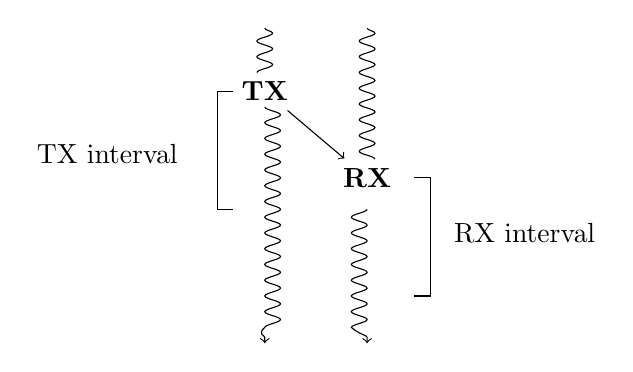
\begin{tikzpicture}
      \draw[->,decorate,decoration={snake,segment length=2mm, amplitude=1mm}]
        (0mm,0mm) -- (0,-5mm)
        (0mm,-8mm) node (TX) {\textbf{TX}} (0,-10mm) --
        (0mm,-40mm);
      \draw (-4mm,-8mm) -- (-6mm,-8mm) -- (-6mm,-23mm) -- (-4mm,-23mm);
      \draw (-20mm,-16mm) node {TX interval};

      \draw[->,decorate,decoration={snake,segment length=2mm, amplitude=1mm}]
        (13mm,0mm) -- (13mm,-16mm)
        (13mm,-19mm) node (RX) {\textbf{RX}} (13mm,-23mm) --
        (13mm,-40mm);
      \draw (19mm,-19mm) -- (21mm,-19mm) -- (21mm,-34mm) -- (19mm,-34mm);
      \draw (33mm,-26mm) node {RX interval};
      \draw[->] (TX) -- (RX);
    \end{tikzpicture}
    \label{fig:enforce:message_windows:tx_first}
  }
  \subfigure[][Intervals overlap; message is sent]{
    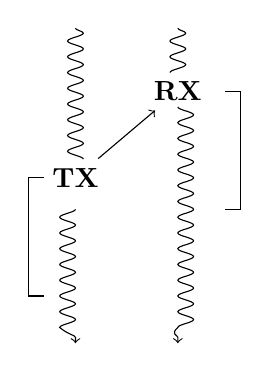
\begin{tikzpicture}
      \draw[->,decorate,decoration={snake,segment length=2mm, amplitude=1mm}]
        (0mm,0mm) -- (0,-16mm)
        (0mm,-19mm) node (TX) {\textbf{TX}} (0,-23mm) --
        (0mm,-40mm);
      \draw (-4mm,-19mm) -- (-6mm,-19mm) -- (-6mm,-34mm) -- (-4mm,-34mm);

      \draw[->,decorate,decoration={snake,segment length=2mm, amplitude=1mm}]
        (13mm,0mm) -- (13mm,-5mm)
        (13mm,-8mm) node (RX) {\textbf{RX}} (13mm,-10mm) --
        (13mm,-40mm);
      \draw (19mm,-8mm) -- (21mm,-8mm) -- (21mm,-23mm) -- (19mm,-23mm);
      \draw[->] (TX) -- (RX);
    \end{tikzpicture}
    \label{fig:enforce:message_windows:rx_first}
  }
  {\hfill}
  \subfigure[][Intervals do not overlap; no message can be sent.]{
    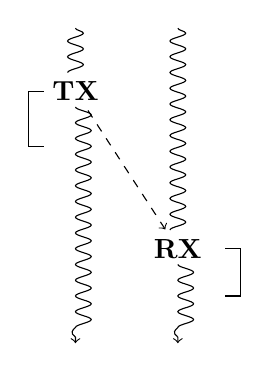
\begin{tikzpicture}
      \draw[->,decorate,decoration={snake,segment length=2mm, amplitude=1mm}]
        (0mm,0mm) -- (0,-5mm)
        (0mm,-8mm) node (TX) {\textbf{TX}} (0,-10mm) --
        (0mm,-40mm);
      \draw (-4mm,-8mm) -- (-6mm,-8mm) -- (-6mm,-15mm) -- (-4mm,-15mm);

      \draw[->,decorate,decoration={snake,segment length=2mm, amplitude=1mm}]
        (13mm,0mm) -- (13mm,-25mm)
        (13mm,-28mm) node (RX) {\textbf{RX}} (13mm,-30mm) --
        (13mm,-40mm);
      \draw (19mm,-28mm) -- (21mm,-28mm) -- (21mm,-34mm) -- (19mm,-34mm);

      \draw[->,dashed] (TX) -- (RX);
    \end{tikzpicture}
    \label{fig:enforce:message_windows:failed}
  }
  \caption{Overlapping TX and RX intervals allow the message to be
    sent, regardless of which operation is ordered first.  If the
    intervals do not overlap then no message can be sent.}
  \label{fig:enforce:message_windows}
\end{figure}

Suppose, for instance, that the interval were set at 20ms.  A
\textbf{TX} operation at time 512ms would then be able to communicate
with an \textbf{RX} operation at 520ms.  This would involve delaying
the transmitting thread by 8ms so that the two operations occur at the
same time.  Similarly, the \textbf{TX} operation could communicate
with an \textbf{RX} at 498ms by delaying the receiving thread by 14ms.
It would not, however, be possible for the \textbf{TX} operation to
communicate with \textbf{RX} operations at 490ms or 540ms, because
those fall outside of the interval.

There are two complications in implementing this behaviour.  First, it
is difficult for a \textbf{TX} operation to look ahead through the
execution to determine how long it should wait for the \textbf{RX}
operation to arrive, or vice versa.  Second, it might be that several
possible partner operations happen during the interval, and the LLI
must decide which to bind to.  In practice, it is not possible to
completely solve these problems and get precisely the desired
behaviour, but it is possible to approximate it reasonably accurately.
{\Implementation} uses the following algorithm to implement the peer
selection part of the \textbf{TX} algorithm; the \textbf{RX} algorithm
is symmetric:

\begin{itemize}
\item[1] Iterate over the global \texttt{rx\_thread} table.  All of
  the entries in this table will be LLIs which are currently at the
  \textbf{RX} state.  Compare the message which this LLI wants to
  transmit to the message which the other LLI wants to receive.  If
  they match, and if any side-condition on the message passes, the
  local LLI completes both message operations.  This means that it
  duplicates both LLIs, copies the necessary state between the two new
  LLIs, advances them past the message operation, and adds them back
  to the appropriate HLIs.
\item[2] Register the current LLI in the global \texttt{tx\_thread}
  table.
\item[3] Sleep for the interval.
\item[4] De-register the current LLI from the \texttt{tx\_thread}
  table.
\item[5] The current LLI now corresponds to the situation where no
  other threads arrived during the interval, and so it has failed and
  should exit.
\end{itemize}

The intent is that when a new \textbf{TX} operation starts, it first
looks for any existing \textbf{RX} operations which are waiting for
it, corresponding to
Figure~\ref{fig:enforce:message_windows:rx_first}.  If it finds any,
it completes both operations, creating new LLIs on both the receive
and transmit side to store its results.  It then goes to sleep waiting
for any further \textbf{RX} operations, corresponding to
Figure~\ref{fig:enforce:message_windows:tx_first}.  If any \textbf{RX}
operations arrive during this window then they will complete both the
\textbf{TX} and \textbf{RX} operations, and so when the sleep
completes the current LLI has no more to do and should exit,
corresponding to
Figure~\ref{fig:enforce:message_windows:failed}\footnote{{\Implementation}
  actually includes an optimisation to avoid creating and destroying
  LLIs unnecessarily in the common case where precisely one peer
  operation is available, but this does not fundamentally alter the
  algorithm and is not shown here.  Likewise, this discussion omits
  the enforcer-internal synchronisation necessary to implement this
  algorithm in a race-free way, to avoid unnecessarily complicating
  the presentation.}.

This algorithm solves the problem of not knowing how long to wait by
always waiting for the maximum possible time, and the problem of not
knowing which of many possible peers to synchronise with by
synchronising with all of them.  That is similar to but not quite
identical to the desired behaviour.  In particular, in the desired
semantics, when a message operation is destined to fail, it should not
wait at all, whereas here failing operations wait for the maximum
possible time.  In other words, the non-deterministic part of the
desired behaviour is correctly implemented, but the non-causal part is
not.  This can sometimes lead to threads delaying for longer than
necessary.  If it were necessary, the correct behaviour could be
achieved using a deterministic replay system\cite{Choi1998} and
techniques similar to a time-travelling debugger\cite{Xu2003}, but at
the probable expense of further impairing performance.  I have not
investigated this at all.

This algorithm assumes that it is possible to delay an arbitrary LLI
for as long as desired, whenever desired, with no adverse effects on
any other part of the program.  This is not entirely true.  In
particular, it is common for a single HLI, and hence a single concrete
program thread, to run multiple LLIs, and it is not possible to delay
one LLI in a thread without also delaying all of the others.  What
effect will these spurious delays have on the program and the
enforcer?  Delaying an unbound LLI is generally safe, as it just
causes the enforcement plan to start a little later, which might lead
to poor performance but will not completely prevent the plan from
succeeding.  Delaying a bound LLI is much more dangerous.  The problem
is that delaying a bound LLI will have knock-on effects on the LLI to
which it has bound, which might cause \emph{that} LLI to fail its part
of the plan, and in the extreme case might completely prevent certain
bugs from reproducing.  To be a little more concrete, suppose that the
plan requires that LLI $l_1$ be delayed but does not impose any delay
on LLI $l_2$, which is in the same HLI, and that $l_2$ is bound to the
LLI $l_3$ in another HLI.  $l_3$ will eventually advance to a point
which requires further communication with $l_2$.  If $l_2$ is
excessively delayed then this message operation will time out, causing
both $l_2$ and $l_3$ to fail.  If this happens consistently then it
might make it impossible to reproduce the bug.

Fortunately, this problem is easily averted by defining the bound
message timeout more carefully.  Rather than timing out after $l_3$
has been waiting for more than time $\tau$, the plan should fail if
$l_2$ takes more than $\tau$ to advance from one message operation to
the next, excluding the time it wastes due to $l_1$'s message
operations.  The HLI can track this information for each LLI, and
$l_3$ adjust its timeout as appropriate.  This avoids the
issue\editorial{Or at least, it does the one case I've actually seen
  this, and I think it does in the general case as well.}.

The interactions with the \textbf{Succ} phase present a further
complication.  The \textbf{Succ} phase sometimes needs to duplicate an
LLI in order to handle ambiguities in the \gls{cfg}, and it must
ensure that the relationships between bound LLIs are correctly
maintained as it does so.  For instance, if $l_1$ and $l_2$ are bound
together and $l_1$ is duplicated to $l_1'$, the HLI should also
duplicate $l_2$ to $l_2'$ so that it can bind $l_1'$ and $l_2'$.  The
alternatives, of leaving $l_1'$ unbound or of binding both $l_1$ and
$l_1'$ to $l_2$, would not allow future message operations to be
correctly implemented in any of the LLIs.

\subsection{Selecting the size of the timeout}
\label{sect:using:timeout_balancing}

\todo{This is quite a lot of words to say something fairly obvious.
  Also, it misses out the most interesting bits of the timeout
  strategy.  And it's possibly in a poor place, as well.}

Up to now, the discussion has assumed that all timeouts are the same,
fixed, size.  This is not always the best possible strategy.  In
particular, it is not always necessary or useful to delay both the
transmit and receive halves of a message operation.  I now show that
one of these delays can usually be omitted, and give a brief
discussion of how to decide which to omit.

Unbound timeouts are generally far more important than bound ones, in
terms of both their effects on the time taken to reproduce the bug and
their effects on the program's performance while running under the
enforcer, as the construction of the plan, and in particular the
selection of side-conditions, ensures that bound messages will only
happen when the target bug has a very high chance of reproducing.
Assume, then, that only unbound delays matter.  Assume further that
the enforcer is only trying to enforce one happens-before graph, that
there are only two threads in the program, and that the delay is small
enough that it does not meaningfully affect the program's behaviour.
There will then be only two message operations to consider, one
\textbf{TX} and one \textbf{RX}, and they will both occur with some
fixed frequency.  Call these frequencies $f_{\mathbf{TX}}$ and
$f_{\mathbf{RX}}$ and call the delays imposed by each operation
$D_{\mathbf{TX}}$ and $D_{\mathbf{RX}}$.

We can then easily estimate the performance cost of the enforcer.  The
fraction of program time spent in those delays is then
$f_{\mathbf{TX}}.D_{\mathbf{TX}} + f_{\mathbf{RX}}.D_{\mathbf{RX}}$,
and that is a reasonable proxy for the overhead $\omega$.

Next, estimate the expected time before the bug is reproduced.  One
way for the bug to reproduce is if the \textbf{TX} might occurs within
$D_{\mathbf{RX}}$ after a \textbf{RX} operation.  In effect, each
\textbf{RX} operation defines a window of size $D_{\mathbf{RX}}$ in
the program's timeline and the bug reproduces if a \textbf{TX} effect
lands in that window.  These windows will cover a fraction
$f_{\mathbf{RX}}.D_{\mathbf{RX}}$ of the timeline, and so, assuming
\textbf{TX}s occur randomly, each will have a probability of
$f_{\mathbf{RX}}.D_{\mathbf{RX}}$ of triggering the bug, giving a bug
reproduction rate of
$f_{\mathbf{TX}}.f_{\mathbf{RX}}.D_{\mathbf{RX}}$.  Symmetrically, the
bug might be reproduced if a \textbf{RX} operation occurs
$D_{\mathbf{TX}}$ after a \textbf{TX} one, giving a reproduction rate
of $f_{\mathbf{TX}}.f_{\mathbf{RX}}.D_{\mathbf{TX}}$.  These are the
only ways in which the bug can reproduce, and so the total
reproduction rate $\rho$ is
$f_{\mathbf{TX}}.f_{\mathbf{RX}}.(D_{\mathbf{RX}} + D_{\mathbf{TX}})$.

The task is now to choose $D$ so as to maximise the reproduction
rate whilst minimising the overhead.  Some simple algebra is
sufficient to show that
\begin{displaymath}
\rho = {\omega}.f_{\mathbf{RX}} + f_{\mathbf{RX}}.D_{\mathbf{RX}}(f_{\mathbf{TX}} - f_{\mathbf{RX}}) = {\omega}.f_{\mathbf{TX}} + f_{\mathbf{TX}}.D_{\mathbf{TX}}(f_{\mathbf{RX}} - f_{\mathbf{TX}})
\end{displaymath}

In other words, if $f_{\mathbf{TX}} > f_{\mathbf{RX}}$ then the
reproduction rate for a given level of overhead is maximised by
setting $D_{\mathbf{RX}}$ as large as possible and $D_{\mathbf{TX}}$
to zero, and conversely when $f_{\mathbf{TX}} < f_{\mathbf{RX}}$.
{\Implementation} therefore keeps a counter of how many times the send
and receive sides of each message operation are attempted; if the send
operation has been attempted more times than the receive one then the
send operation delay is set to zero, and otherwise the receive delay
is set to zero.  The other delay is set to some user-configured
constant.

\todo{Maybe discuss that this can affect chance of reproducing as well
  as performance?  It's true, I just don't have a great deal
  interesting to say about it.}

\section{Implementing the $\smLoad{}$ operation}

The side-condition placement algorithm\editorial{Or whatever.} removes
all of the happens-before $\happensBeforeEdge$ queries from the
side-condition, and most of the remaining parts of the {\StateMachine}
expression language are simple to implement.  The only exception is
the $\smLoad{}$ expression, which is defined to return the initial
contents of memory at a given address.  This is not entirely
well-defined in a running program with multiple threads.  Even worse,
the address itself might not become evaluatable until one or both of
the threads involved in the crash have been running in the interpreter
for some time.  {\Implementation} only implements an approximation of
the desired behaviour: it captures the contents of memory at the point
the address becomes evaluatable, rather than trying to capture any
kind of initial value.  In practice, this is usually sufficient,
because the address usually becomes evaluatable to the interpreter at
the same time as it becomes evaluatable to the program itself, and so
the program will usually not have been able to access the memory
before this point, and so even when the captured value differs from
the initial value it will not usually matter.

A second, less severe, problem is that the address, when it becomes
evaluatable, might refer to invalid memory, even when the original
program is guaranteed to only ever access valid memory.  The problem
here is that the side-condition placement strategy can sometimes, in
effect, lift memory accesses past control-flow branches, and if that
control-flow branch was a test of the validity of the pointer then the
side-condition might involve invalid pointers.  {\Implementation}
solves this problem by simply catching page faults generated while
evaluating side conditions.  If any such faults occur then the
relevant LLI is considered to have failed.

